\documentclass[12pt,a4paper,twoside]{article}
\usepackage{labor}
\begin{document}

%fill for cover and header creation
\newcommand\laboratorynumber{2}
\title{Interferometer}
\newcommand\supervisor{Ditlbacher, Harald}
\newcommand\groupnumber{42}

\newcommand\participantonelastname{Eisner}
\newcommand\participantonefirstname{Nico}
\newcommand\participantoneid{12214121}
\newcommand\participanttwolastname{Waldl}
\newcommand\participanttwofirstname{Philip}
\newcommand\participanttwoid{12214120}
\author{\participantonelastname \ \& \participanttwolastname}

\newcommand\degreeid{UB 033 678}
\newcommand\semester{23WS}
\date{01.12.2023}

%select correct course title
%\newcommand\coursetitle{Einführung in die \\ physikalischen Messmethoden}
%\newcommand\coursetitle{Laborübungen 1: \\ Mechanik und Wärme}
\newcommand\coursetitle{Laborübungen 2: \\ Elektrizität, Magnetismus, Optik}
%\newcommand\coursetitle{Fortgeschrittenen Praktikum 1: \\ Technische Physik}
%\newcommand\coursetitle{Fortgeschrittenen Praktikum 2: \\ Allgemeine Physik}

%\begin{titlepage}
   \begin{center}
       \begin{figure}[H]
            \begin{minipage}[h]{30mm}
                \centerline{
\includegraphics[height=15mm]{cover_nudes/tugraz.png}}
            \end{minipage}
            \hfill
            \begin{minipage}[h]{30mm}
                \centerline{
\includegraphics[height=15mm]{cover_nudes/nawi_graz.png}}
            \end{minipage}
            \hfill
            \begin{minipage}[h]{30mm}
                \centerline{
\includegraphics[height=15mm]{cover_nudes/uni-graz.png}}
            \end{minipage}
        \end{figure}
        
        \large{\emph{Institut für Experimentalphysik der Technischen Universität Graz \\
        \& Institut für Physik der Universität Graz}} \\
        \vspace{5mm}
        
        {\Huge \textbf{\coursetitle}}
        \vspace{5mm}
        
        {\huge \laboratorynumber: \thetitle}
    \end{center}
    
    \vfill
    
    \begin{table}[H]
        \LARGE
        \centering
        \begin{tabular}{r l}
            Betreuer:       & \supervisor \\
            Gruppennummer:  & \groupnumber \\
            \\
            Name:           & \participantonelastname, \participantonefirstname \\
            Matrikelnummer: & \participantoneid \\
            Name:           & \participanttwolastname, \participanttwofirstname \\
            Matrikelnummer: & \participanttwoid \\
            \\
            Kennzahl:       & \degreeid \\
            Datum:          & \semester \ | \thedate
        \end{tabular}
    \end{table}
    \vspace{4cm}
\end{titlepage}
\clearpage
\setcounter{page}{1}

%\maketitle %short title alternative

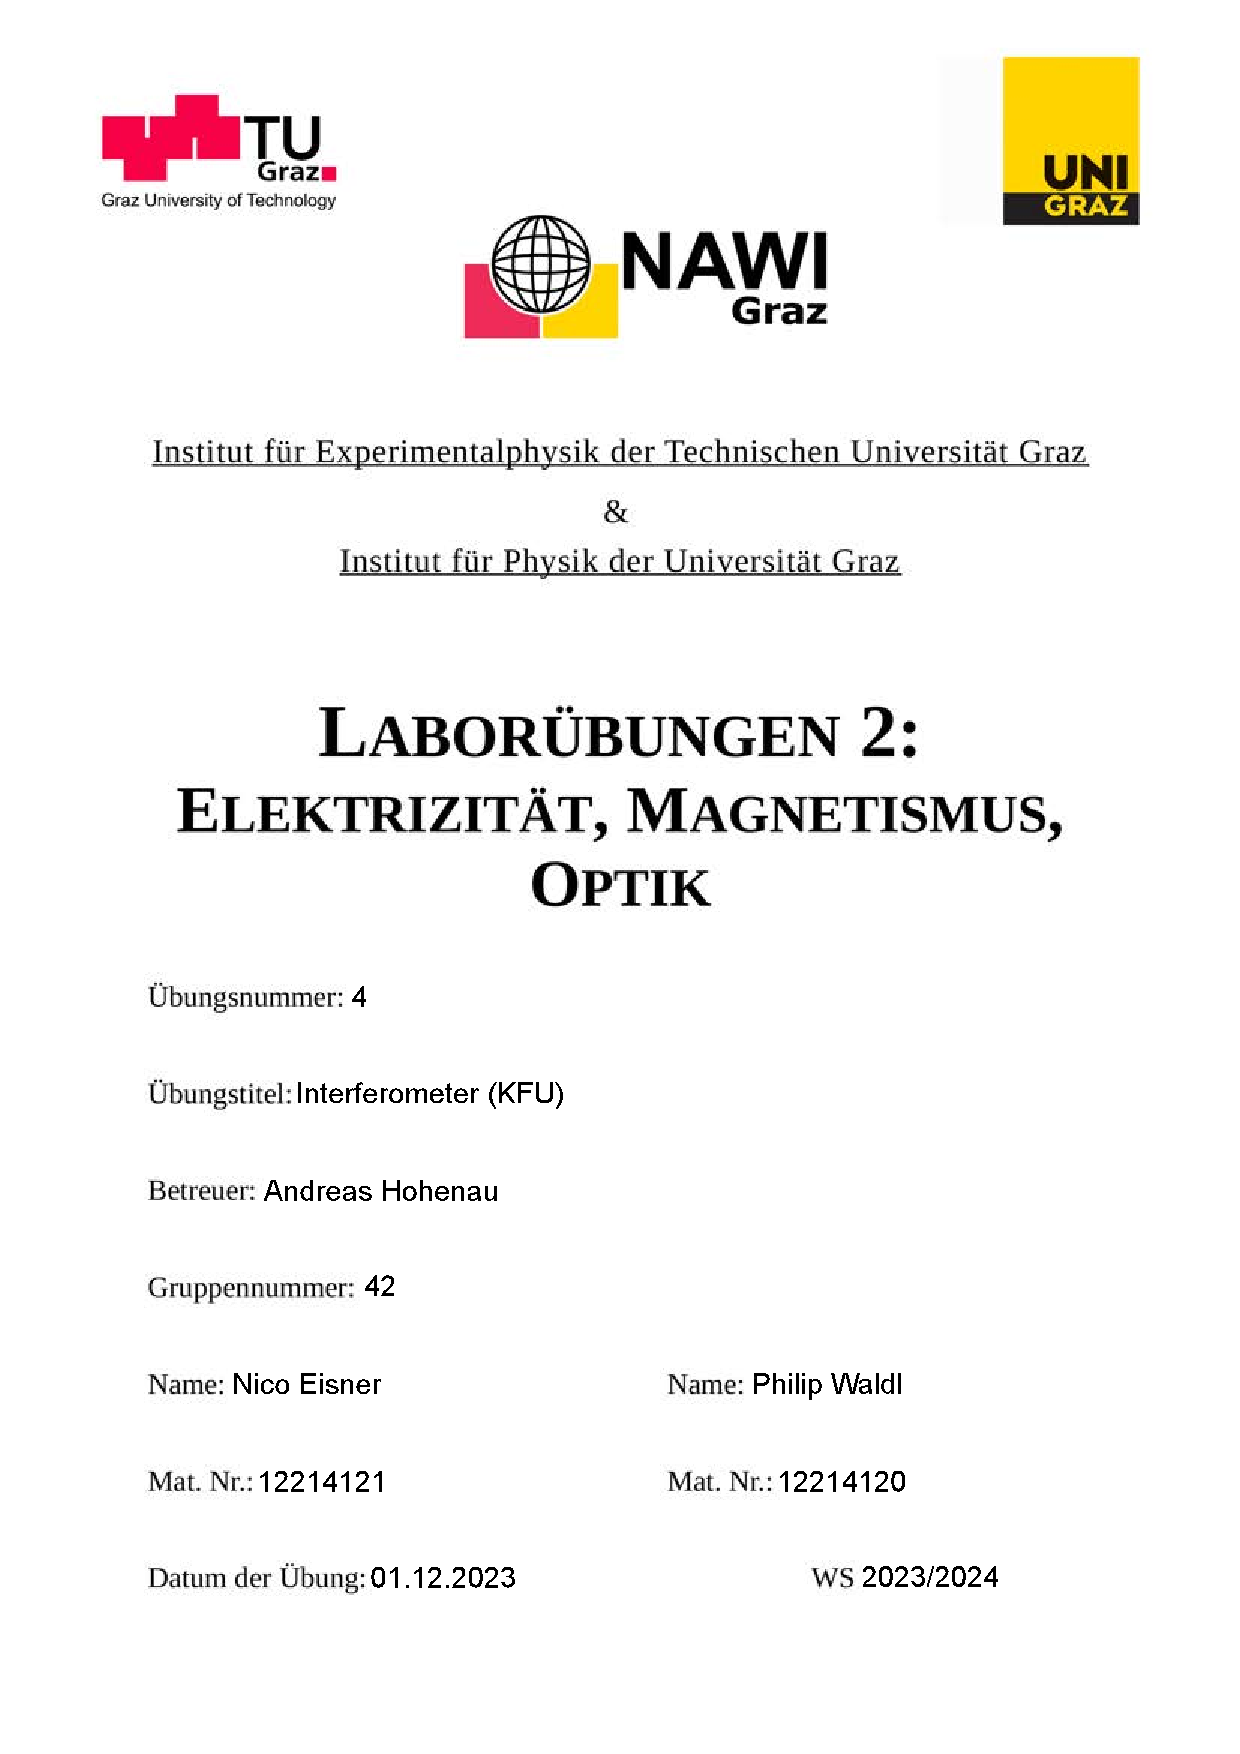
\includepdf[pages={1}]{../Deckblätter/Deckblatt_Interferometer.pdf}

\tableofcontents
\newpage

\section{Aufgabenstellung} %jo beschreibn wos gmocht host ------------------------------
Das Experiment Interferometer gilt es folgende vier Aufgaben durchzuführen. 
\\
\\
Der erste Teil besteht darin, den Einfluss der Größe einer Lichtquelle auf das Interferenzenmuster eines Doppelspaltes zu Demonstrieren und auch zu Erklären. 
\\
Im zweiten Teil wird der Einfluss der spektralen Breite des Lichtes, wie im ersten Teil, auf das Interferenzenmuster eines Doppelspaltes zu Demonstrieren und zu Erklären. 
\\
Im dritten Teil wird mithilfe des Doppelspalt-Interferenzenmusters die Dicke einer Kunststoffschichicht bestimmt. 
\\
Der vierte und letzte Teil besteht aus der Bestimmung der Größe der Lichtquelle bei welcher für Doppelspalten mit unterschiedlichem Spaltabstand das Licht noch räumlich kohärent ist. 
\\
\\
Alle Informationen und Methodiken wurden uns von der Technischen Universität bereitgestellt \cite{teachcenter2}. 

\section{Voraussetzungen \& Grundlagen} %Grundlagen erklären, Formeln mit erklärung
Ein Interferenzmuster entsteht durch Überlagerung der Wellenfronten. Sendet man monochromatisches Licht aus einer Lichtquelle durch eine Sammellinse, so entstehen kugelförmige Wellenfronten. 
Treten diese kugelförmige Wellenfronten durch einen Doppelspalt, so treten aus dem Spalt phasengleiche kugelförmige Wellenfronten aus. 
Treffen dabei die Wellenfronten (Maxima und Minima) aufeinander, addieren sich diese konstruktiv. So entstehen größere Maxima und kleinere Minima. 
Durch phasengleichen Austritt der Wellenfronten aus dem Doppelspalt entstehen Interferenzen bei den Winkeln $\theta$ wo der Phasenverschub ein Vielfaches von 2$\pi$ ist. 
Dies geschieht, wo die Differenz der Strecke $\Delta s$ ein Vielfaches der Wellenlänge $\lambda$ beträgt. m ist die Zahl der Ordnung. 

\begin{equation}
    \label{eq:beugung am doppelspalt}
    \centerline{$\Delta s = dsin(\theta_m) = m\lambda$}
\end{equation}

\noindent
Durch die Brennweite und den Abstand zum Doppelspalt der Linse L2 kann der absolute Abstand des 0-ten bis zum m-ten Maxima berechnet werden. m ist die Zahl der Ordnung. 

\begin{equation}
    \label{eq:grundlagen 2}
    \centerline{$b_m = f_2 tan$ $arcsin(\frac{m \lambda}{d})$}
\end{equation}

\noindent
Fügt man in den Strahlengang nun ein Material (Polyacrylat) mit unterschiedlichen Brechungsindex $n$ und physikalischer Dicke $t$ ein, so ändert sich auch die Lichtgeschwindigkeit im Medium. 
Dadurch braucht der Lichtstrahl länger um abgebildet zu werden. Durch diese Dauer verschiebt sich das 0-te Maximum. Es befindet sich daher nichtmehr bei $\Delta s_0 = 0$ sondern bei: 

\begin{equation}
    \label{eq:verschiebung}
    \centerline{$\Delta s_0 = d sin(\theta_0) + tn_2 - tn_1$}
\end{equation}

\begin{figure}[H]
    \centering
    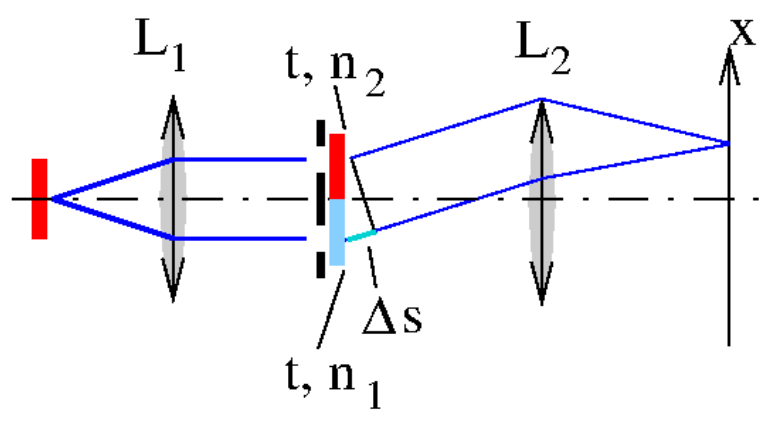
\includegraphics[width=0.6\linewidth]{nudes/verschiebung.png}
    \caption{Beugung am Doppelspalt mit Schichten unterschiedlicher Brechungsindizes $n$ und Stärken $t$. Entnommen aus Skriptum Interferometer Seite 10, Abbildung 7 \cite{teachcenter2}. }
    \label{fig:verschiebung}
\end{figure}

\noindent
Durch verschiebung der Lichtquelle verschiebt sich auch das Interferenzmuster. Die Lichtquelle ist im idealen fall Punktförmig, in diesem Fall besitzt sie eine gewisse Ausdehnung $2w$. 
Für jeden Punkt der Lichtquelle entstehen Interferenzmuster welche sich überlagern. Man spricht hier von räumlicher Kohärenz, wenn unterschiedlichen Lichtquellen unterschiedliche Nullmaxima haben. 
Durch die Spaltblende wird dies auf eines begrenzt. \\
In den später beobachtbaren Interferenzmustern wird dadurch der Kontrast $K$ verringert. Dieser lässt sich mit folgender Formel bestimmen. Dabei ist $I$ die Intensität. 

\begin{equation}
    \label{eq:Kontrast}
    \centerline{$K = \frac{I_{max} - I_{min}}{I_{max} + I_{min}} $ \\ $\Delta K = \vert \frac{\partial K}{\partial I_{max}} * \Delta I_{max} \vert + \vert \frac{\partial K}{\partial I_{min}} * \Delta I_{min} \vert$} %= \vert \frac{sin(2 \pi \frac{d}{\lambda} \frac{w}{f_1})}{2 \pi \frac{d}{\lambda} \frac{w}{f_1}} \vert$}
\end{equation}

\noindent
Für den theoretischen Verlauf bzw. Erwartungswert des Kontrastes wird die folgende Formel verwendet. Dabei ist $d$ der Doppelspalt, $\lambda$ die Wellenlänge, welche durch den Bandpassfilter begrenzt wird. $2w$ ist dabei die Breite der Lichtquelle und $f$ die Brennweite. 

\begin{equation}
    \label{eq:Kontrasttheorie}
    \centerline{$K = \vert \frac{sin(2 \pi \frac{d}{\lambda} \frac{w}{f_1})}{2 \pi \frac{d}{\lambda} \frac{w}{f_1}} \vert$}
\end{equation}


\section{Versuchsanordnung} %mit skizze kurz beschreiben ------------------------------
Der Versuch ist wiefolgt aufgebaut. 

\begin{figure}[H]
    \centering
    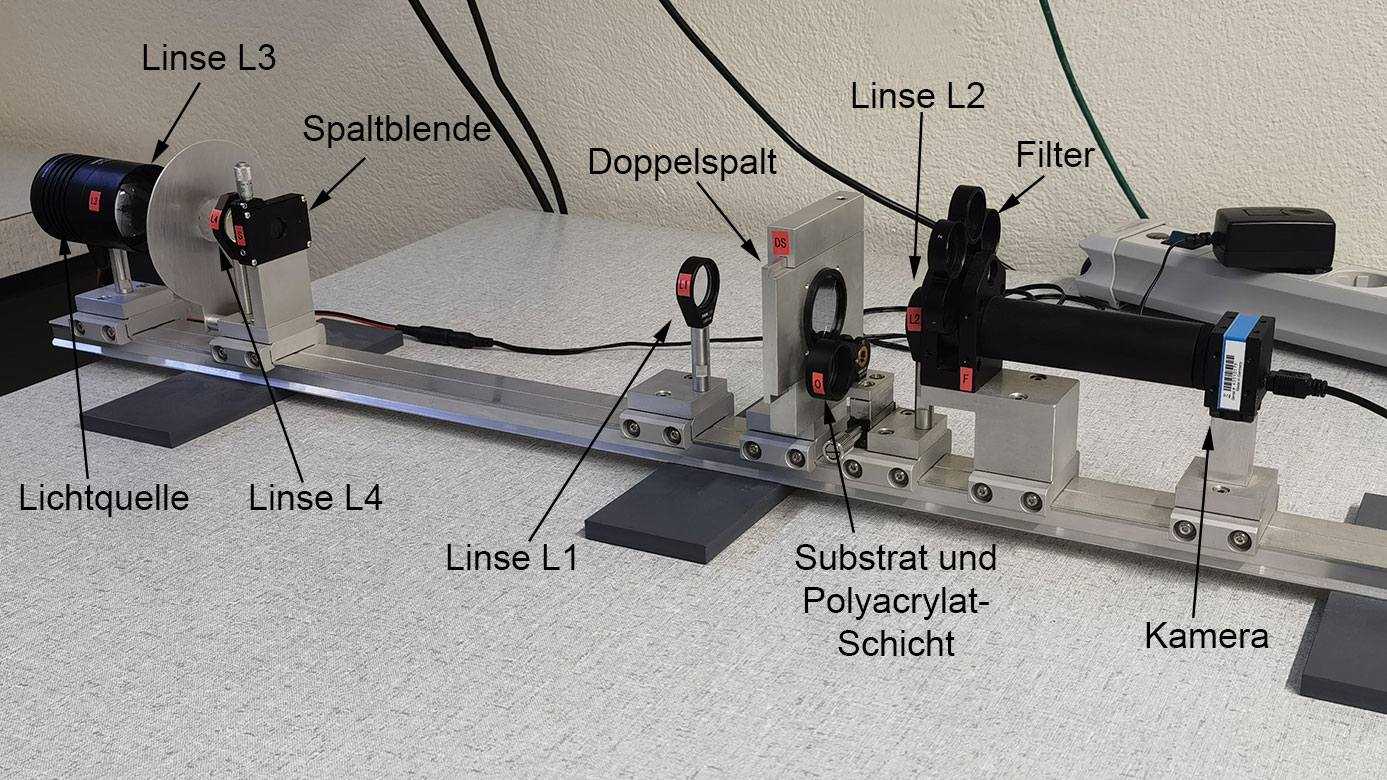
\includegraphics[width=0.6\linewidth]{nudes/aufbau.jpg}
    \caption{Aufbau des Versuches.}
    \label{fig:aufbau}
\end{figure}

\noindent
Die Lichtquelle wird über eine einstellbare Spaltblende geleitet. Durch diese lässt sich die Größe der Lichquelle einstellen. 
Durch die Linse L1 werden die Lichtstrahlen parallelisiert bevor sie auf den Doppelspalt treffen. 
Nach dem Doppelspalt trifft das Licht auf ein Substrat. In diesem befindet sich die Polyacrylat Schicht. 
Nach diesem trifft das Licht auf die Linse L2, welche das Licht auf den Kamerasensor lenkt. Zwischen Linse L2 und Kamera befindet sich noch ein Filterrad, durch welches sich verschiedene Filter hinzugefügt werden können. 


\section{Geräteliste} %jo holt a listn ------------------------------

    \begin{table}[H]
        \centering
        \caption{Im Versuch verwendete Geräte und Utensilien. Bei Geräten, dessen Unsicherheit nicht auffindbar ist, wird die Unsicherheit implizit angenommen oder die Ableseunsicherheit genommen. }
        \label{tab:geraete}
        \begin{tabular}{| l | l | l |}
            \hline
            Gerät    & Gerätenummer  & Unsicherheit \\
            \hline
            Lampe & Thorlabs QTH10/M & {n.a} \\
            Sammellinsen & Thorlabs LMR1/M & $\pm 0.5 mm$ \\
            Spaltblende & Thorlabs & $\pm 0.05 mm$ \\
            Doppelspalte (130.0, 230.0, 430.0)$\mu m$ & Mitutoyo & $\pm 0.5 \mu m$ \\
            Substrat \& Polyacrylat & Thorlabs TRF90/M & {n.a} \\
            Kamera & {n.a} & {n.a} \\
            Langpassfilter  & {n.a} & {n.a} \\
            Bandpassfilter $\lambda = 633 nm$& {n.a} & $\pm = 0.5 nm$ \\
            IC Capture & {n.a} & {n.a} \\
            Fiji ImageJ & {n.a} & {n.a} \\
            \hline
        \end{tabular}
    \end{table}


\section{Versuchsdurchführung \& Messergebnisse} %nachvollziehbar und klar dargestellt ------------------------------
Der Versuch ist wie in Abbildung \ref{fig:aufbau} bereits aufgebaut. Die Datenauslese erfolgt über den UniPC mit IC Capture. 
Bei den Aufnamen ist es wichtig, vorher die Belichtungszeit einzustellen, so dass kein Pixel die Intensität von 255 überschreitet, da es ansonsten zu fehlerhaften Messdaten kommt. 
Mithilfe des Histogrammes wird geprüft, dass die Belichtungszeit dementsprechend gewählt wird. Die rechte Seite des Histogrammes sollte dabei nie die Intensität von 255 erreichen. 

\begin{figure}[H]
    \centering
    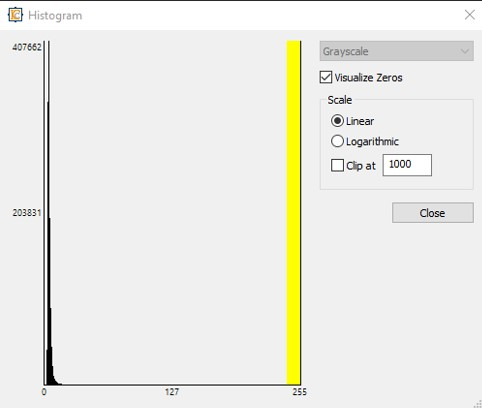
\includegraphics[width=0.6\linewidth]{nudes/histogramm.jpg}
    \caption{Screenshot des Histogrammes. }
    \label{fig:histogram}
\end{figure}

\noindent
Anfangs gilt es den Öffnungsabstand der Spaltblende zu bestimmen. Dazu wird der 230.0 $\mu m$ Doppelspalt verwendet und auf den Filterrad wird kein Filter zugeschalten. 
Der Spalt wird vollständig geschlossen. Durch langsames öffnen, bis ein Bild auf der Kamera zu erkennen ist wird der Offset bestimmt. Die Anzeige der Schraube wird abgelesen und bei den folgenden Werten miteinberechnet. 
Die Abweichung beträgt $(0.35 \pm 0.05) mm$, das bedeutet, bei den folgenden Werten muss ein Offsetwert von 0.15mm dazugerechnet werden. 

\subsection{Teil 1}
Im ersten Teil wird mit dem 430.0 $\mu m$ Doppelspalt und dem Bandpassfilter gearbeitet. 
Der Lichtspalt der Spaltblende $2w$ wird von einer Öffnung von 0.10 mm bis 1.4 mm geöffnet in 0.10 mm Schritten. Die Interferenzmuster werden dabei gespeichert. 
In der folgenden Abbildung werden die Interferenzmuster dargestellt, dabei ist das Oberste bei 1.4 mm. Die Öffnungen $2w$ sind absteigend. 

\begin{figure}[H]
    \centering
    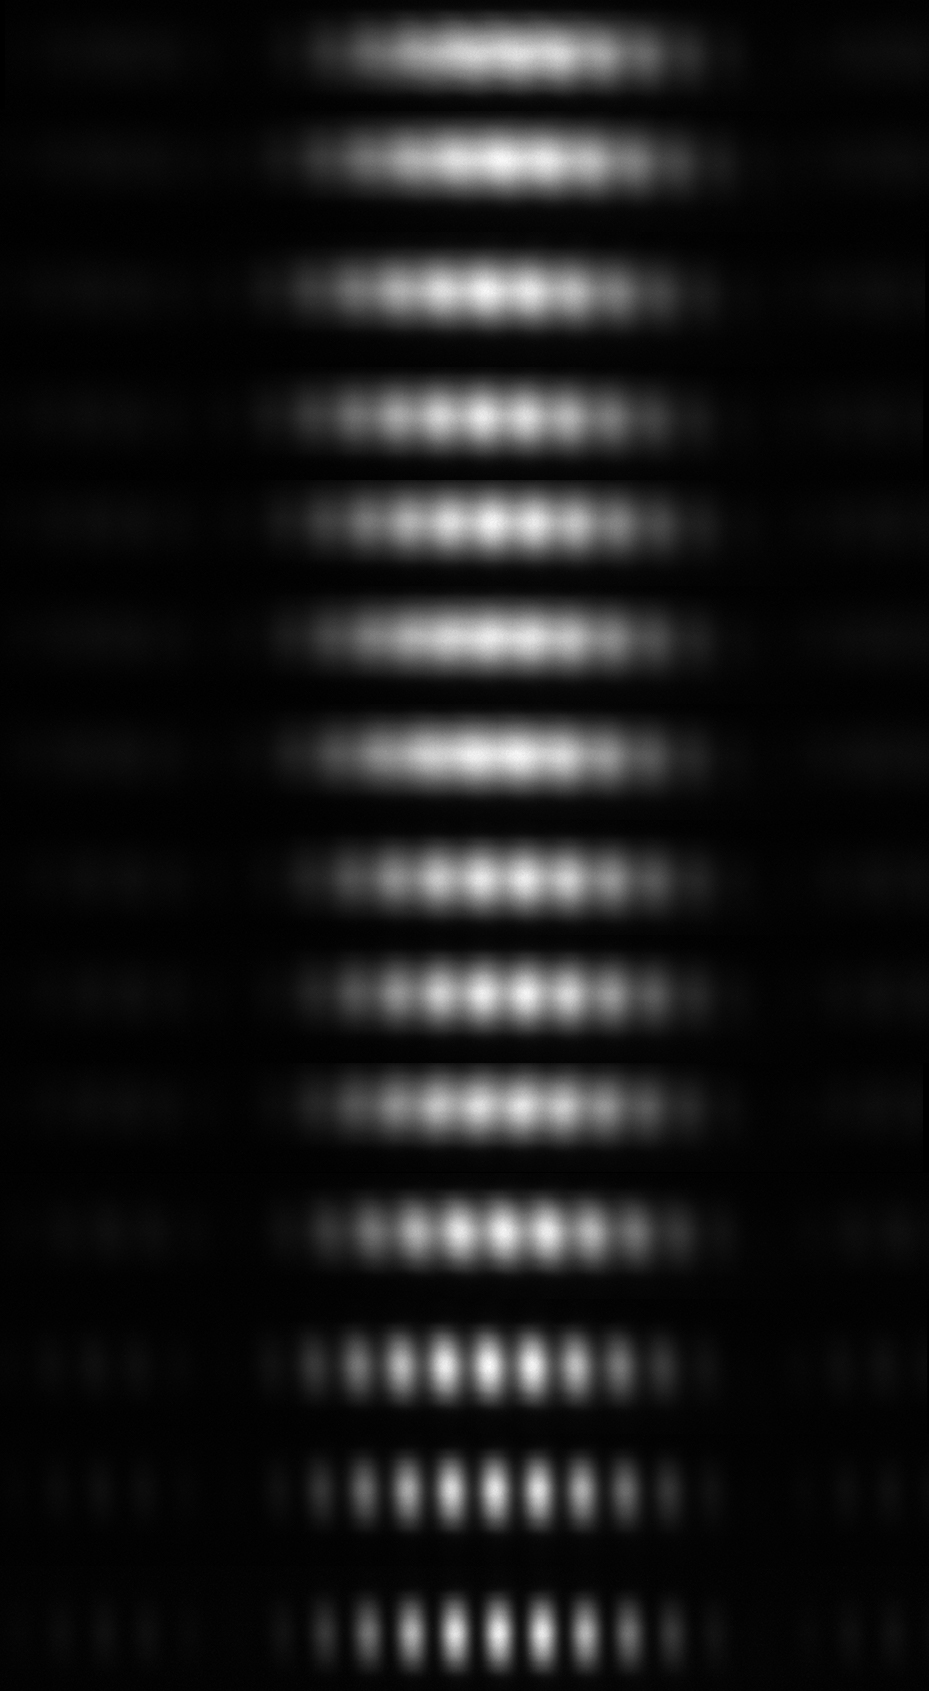
\includegraphics[width=0.6\linewidth]{nudes/aufgabe 1.jpg}
    \caption{Interferenzmuster bei einer Öffnung $2w$ von 0.1 mm (unten) bis 1.4 mm (oben). }
    \label{fig:aufgabe 1}
\end{figure}

\subsection{Teil 2}
Im zweiten Teil bleibt der Doppelspalt mit 430.0 $\mu m$. Es wird ein Interferenzmuster mit dem Langpassfilter, den Bandpassfilter und eines ohne Filter aufgenommen. 
Dazu schließt man die Spaltblende und mit den Bandpassfilter wird die Spaltblende geöffnet, bis ein kontrastreiches Interferenzmuster erkennbar ist. 

\begin{figure}[H]
    \centering
    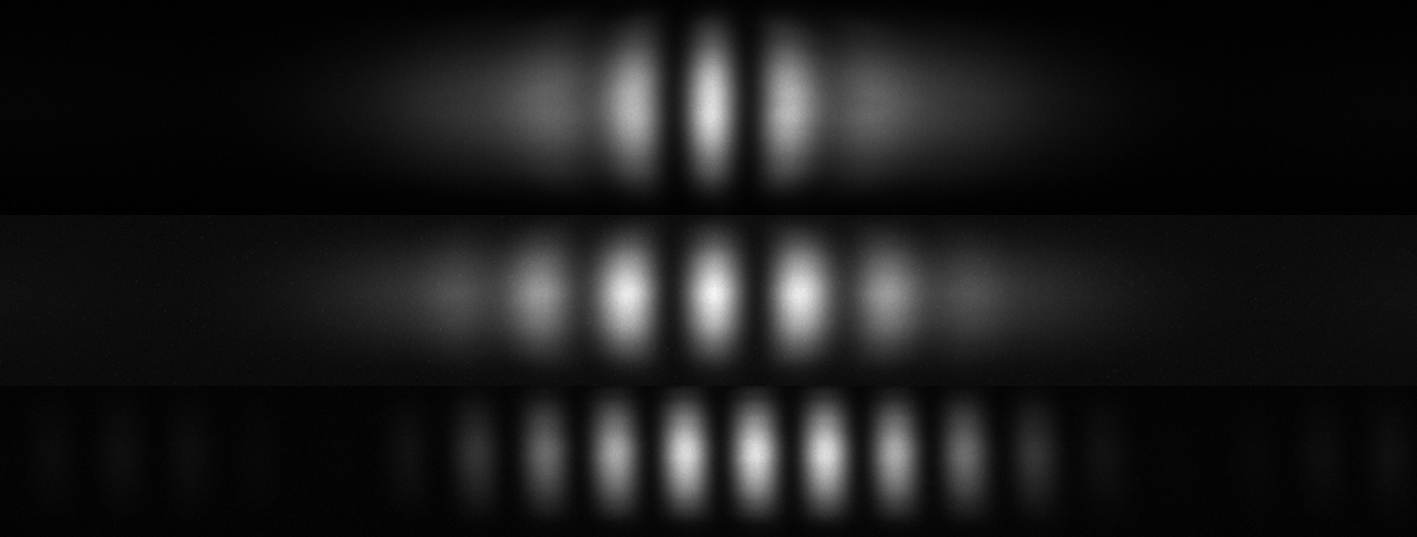
\includegraphics[width=0.6\linewidth]{nudes/aufgabe 2.jpg}
    \caption{Interferenzmuster mit verschiedenen Filter. Ohne Filter (oben), Langpassfilter (mitte), Bandpassfilter (unten) }
    \label{fig:aufgabe 2}
\end{figure}

\subsection{Teil 3}
Im dritten Teil gilt es die dicke einer Polyacrylatschicht zu bestimme. Dazu wird derselbe Doppelspalt mit 430.0 $\mu m$ verwendet. Das Filterrad wird so eingestellt, dass kein Filter im Strahlengang ist. 
Die Probe wird in den Strahlengang gegeben. Durch drehen der Justageschraube lässt sich die Probe verschieben, so dass einmal das unbeschichtete Substrat im Strahlengang ist und einmal die Polyacrylat Schicht. 
Es wird jeweils ein Bild des Beugungsmusters aufgenommen. Einmal mit Verschiebung und einmal vor Verschiebung und einmal dannach. Bei überschreiten der Schichtgrenze zwischen Substrat und Polyacrylat ist ein sprunghafter Verschub des Beugungsmusters zu beobachten. 
%Anschließend wird noch ohne Substrat und ohne Polyacrylat ein Referenzbild mit dem Bandpassfilter aufgenommen. 
Aus Teil 2 wird noch ein Referenzbild mit dem Bandpassfilter hinzugefügt. 

\begin{figure}[H]
    \centering
    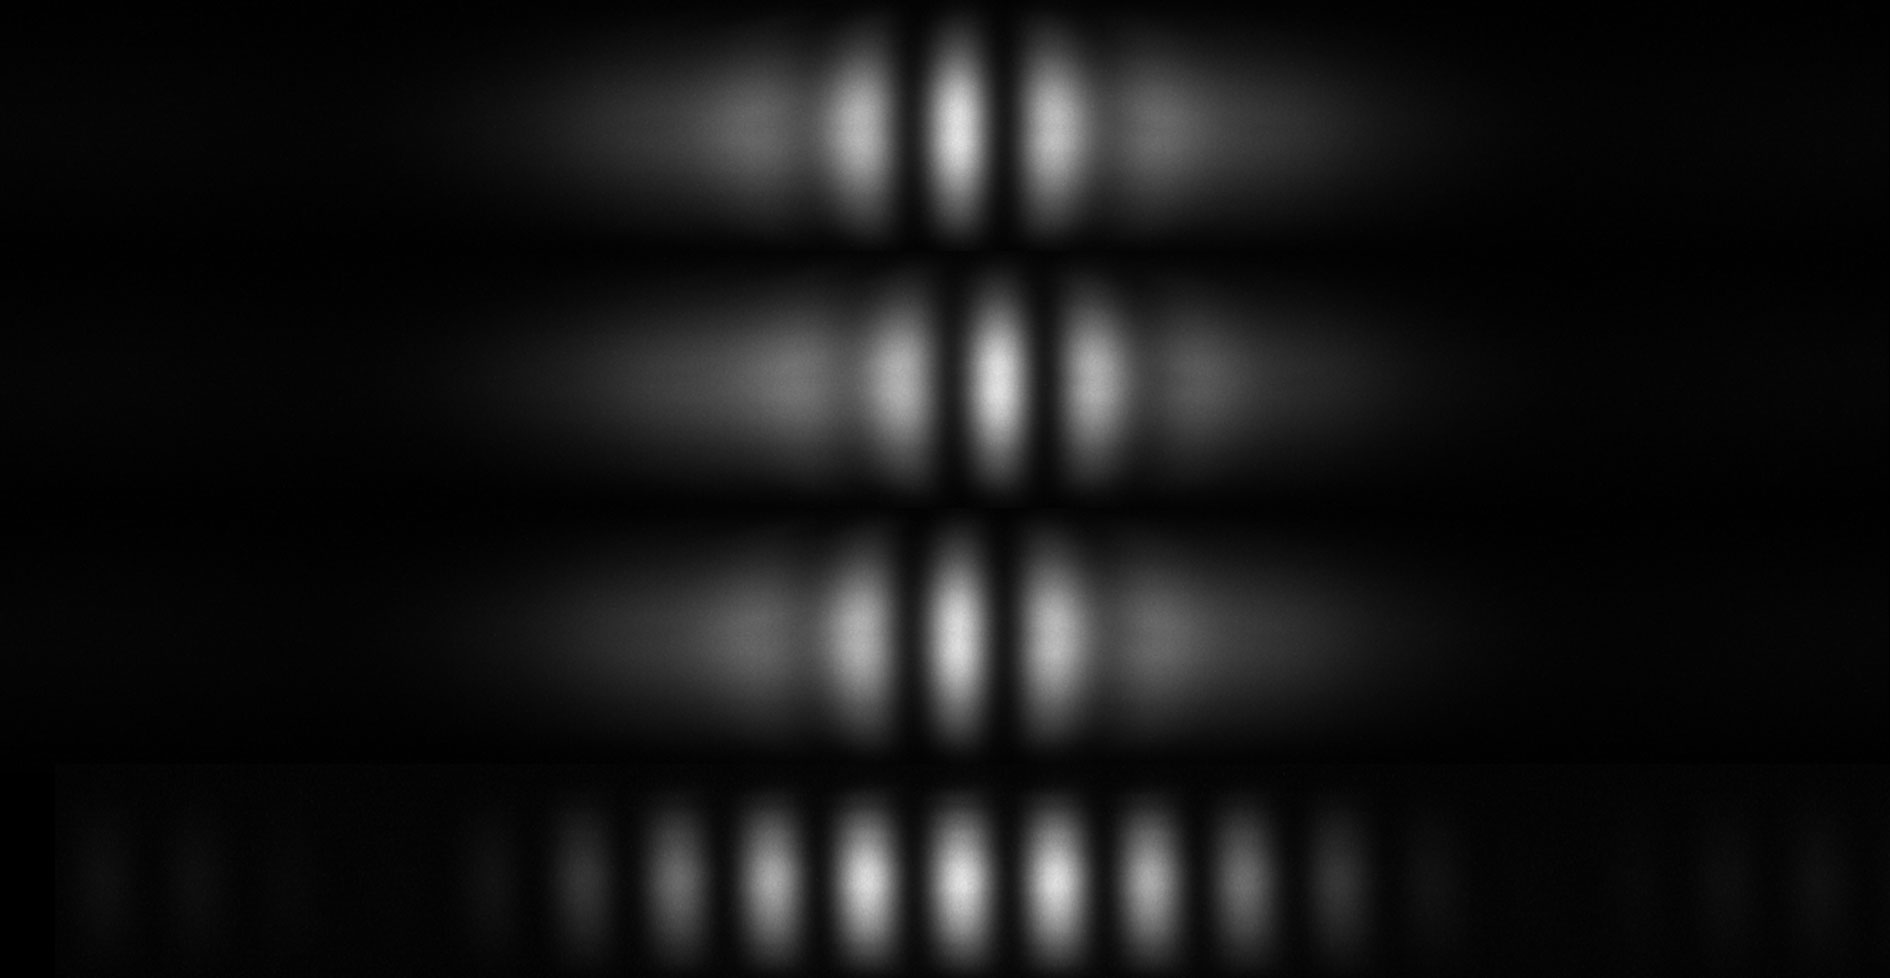
\includegraphics[width=0.6\linewidth]{nudes/aufgabe 3 neu.jpg}
    \caption{Beugungsmuster mit Substrat vor Schicht (oben), Polyacrylat Schicht (mitte) und Substrat nach Polyacrylat Schicht (unten). Referenzbild mit Bandpassfilter (unten). }
    \label{fig:aufgabe 3}
\end{figure}

\subsection{Teil 4}
Wie im vorherigen Teil bleibt der Bandpassfilter im Strahlengang. 
Der 130.0 $\mu m$ Doppelspalt wird in den Strahlengang gesetzt. Die Spaltblende wird geschlossen und dann langsam geöffnet, bis ein Interferenzmuster sichtbar wird. 
Durch weiteres öffnen verschwimmt das Interferenzmuster vollständig. Der Kontrast ist jetzt minimal. Diese Öffnung der Spaltblende wird notiert. 
Dies wird für die weiteren Doppelspalte wiederholt.  

\begin{figure}[H]
    \centering
    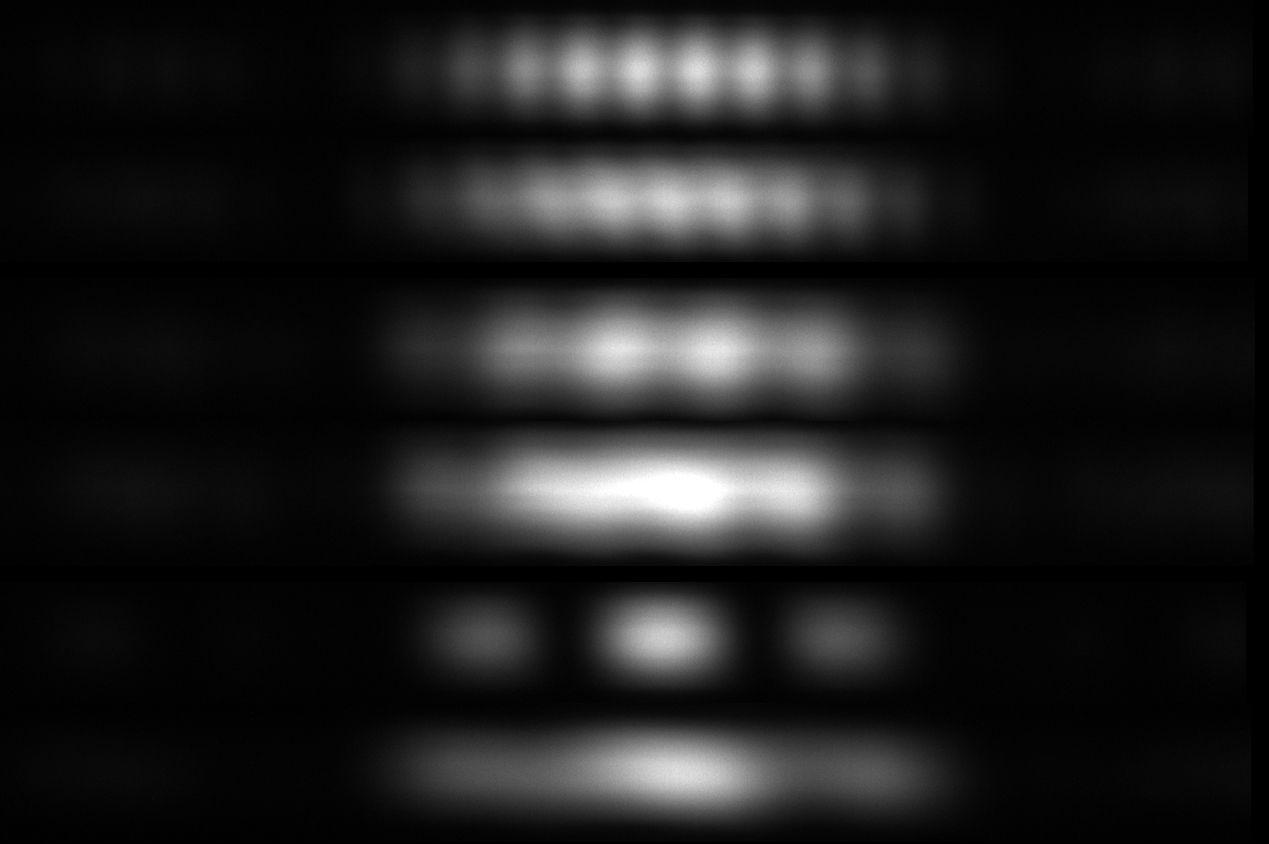
\includegraphics[width=0.6\linewidth]{nudes/aufgabe 4.jpg}
    \caption{Interferenzmuster aller Doppelspalte. Die beiden oberen sind die des 430.0 $\mu m$ Spaltes, die mittleren die des 230.0 $\mu m$ Spaltes und die unteren beiden die des 130.0 $\mu m$ Spaltes. 
    Dabei sind jeweils die ersten die mit minimalem Kontrast und die zweiten mit gutem Kontrast zum vergleich. }
    \label{fig:aufgabe 4}
\end{figure}

\begin{table}[H]
    \centering
    \caption{Öffnungen der  Spaltblende $2w$ bei verschwommenen Interferenzmuster (minimaler Kontrast) für die verschiedenen Doppelspalte $d$. }
    \label{tab:öffnungen}
    \begin{tabular}{| l | l |}
        \hline
        d $\pm 0.5$ / $\mu m $ & 2w $\pm 0.05$/ mm \\
        \hline
        430.0 & 0.85  \\
        230.0 & 1.02  \\
        130.0 & 1.65  \\
        \hline
    \end{tabular}
\end{table}

\section{Auswertung und Unsicherheitsanalyse} %Nicht nur zahlen angeben ------------------------------

In der Auswertung werden zur erhöhten Genauigkeit durchgehend ungerundete Werte bis zu den Endergebnissen verwendet und nur zur Darstellung gerundet. \\
Zur Berechnung der Unsicherheiten wird, wenn nicht anders angegeben, die Größtunsicherheitsmethode verwendet.
\\
\\
Die mit der Kamera aufgenommenen Interferenzmuster werden mithilfe der Software ''ImageJ'' analysiert. 
Dabei werden Intensitätsprofile erstellt, welche als CSV-Datei exportiert werden. 

\begin{figure}[H]
    \centering
    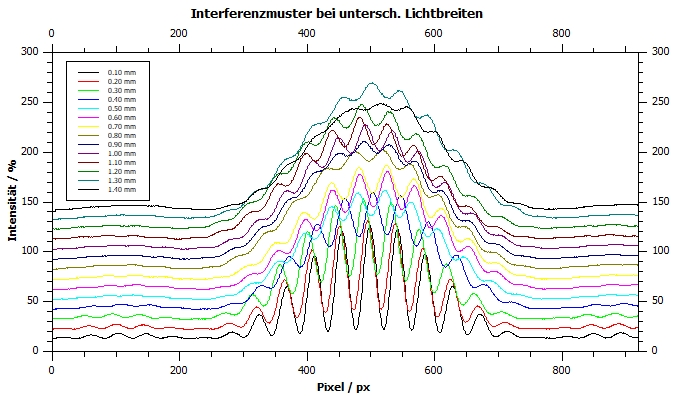
\includegraphics[width=0.6\linewidth]{nudes/aufgabe 1 plot.jpg}
    \caption{Interferenzmuster bei verschiedenen Spaltbreiten (Lichtquellengröße). Zur Darstellung wurden die Daten vertikal getrennt. }
    \label{fig:aufgabe 1 plot}
\end{figure}

\noindent
Aus den CSV-Dateien wird das Intensitätsmaximum und Minimum ausgelesen. Für das Minimum wird der linke und rechte Wert gemittelt. Eingesetzt in die Formel \ref{eq:Kontrast} erhält man den Kontrast pro Spaltbreite $2w$. 
Der Wert des Kontrastes wurde anschließend nochmal mit 100 multipliziert, sodass man den Wert in Prozent erhält. 
Die Unsicherheiten der Intensitäten sind dabei die Ableseunsicherheiten in Qti Plot. 

\begin{table}[H]
    \centering
    \caption{Kontrast $K$ pro Spaltbreite 2w (Lichtquellengröße) mit dazugehörigen Intensitätsmaximum $I_{max}$ und Minimum $I_{min}$.  }
    \label{tab:kontrast}
    \begin{tabular}{| l | l | l | l |}
        \hline
        Spaltbreite 2w $\pm 0.05$ / mm & $I_{max}$ $\pm 0.0005 $ / \% & $I_{min}$ $\pm 0.0005$ / \% & K / \% \\
        \hline
        1.40 & 108.9691 & 101.9662  & 3.4   $\pm$ 1.0   \\
        1.30 & 139.5772 & 122.5767  & 6.5   $\pm$ 0.8   \\
        1.20 & 127.7342 & 105.2003  & 9.7   $\pm$ 0.9   \\
        1.10 & 124.6181 & 96.2478   & 12.9  $\pm$ 1.0   \\
        1.00 & 127.3105 & 100.1558  & 12.0  $\pm$ 0.9   \\
        0.90 & 120.5227 & 107.3559  & 5.8   $\pm$ 0.9   \\
        0.80 & 122.6704 & 106.3307  & 7.2   $\pm$ 0.9   \\
        0.70 & 116.7189 & 86.6813   & 14.8  $\pm$ 1.0   \\
        0.60 & 120.3311 & 83.7664   & 18.0  $\pm$ 1.0   \\
        0.50 & 111.3533 & 85.0506   & 13.4  $\pm$ 1.1   \\
        0.40 & 119.9133 & 76.2207   & 22.3  $\pm$ 1.1   \\
        0.30 & 122.7907 & 46.0073   & 46    $\pm$ 2     \\
        0.20 & 111.6321 & 22.1324   & 67    $\pm$ 2     \\
        0.10 & 116.5771 & 11.7119   & 82    $\pm$ 2     \\
        \hline
    \end{tabular}
\end{table}

\begin{figure}[H]
    \centering
    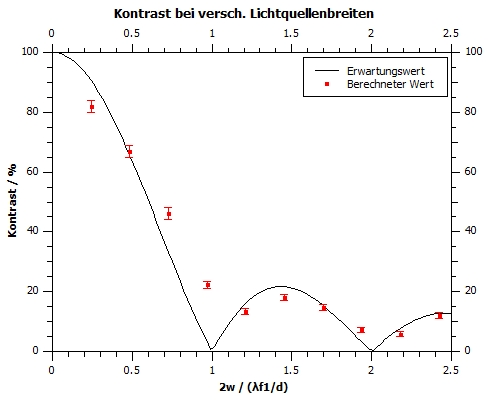
\includegraphics[width=0.6\linewidth]{nudes/kontrast.jpg}
    \caption{Kontrast bei versch. Lichtquellenbreiten. Theoretisch berechneter Wert laut Formel \ref{eq:Kontrasttheorie} im vergleich zu den berechneten Werten aus Tabelle \ref{tab:kontrast}. }
    \label{fig:aufgabe 1 kontrast}
\end{figure}

\subsection{Teil 2}
Die aufgenommenen Interferenzmuster der verschiedenen Filter werden mit ImageJ analysiert und als CSV-Datei exportiert. 

\begin{figure}[H]
    \centering
    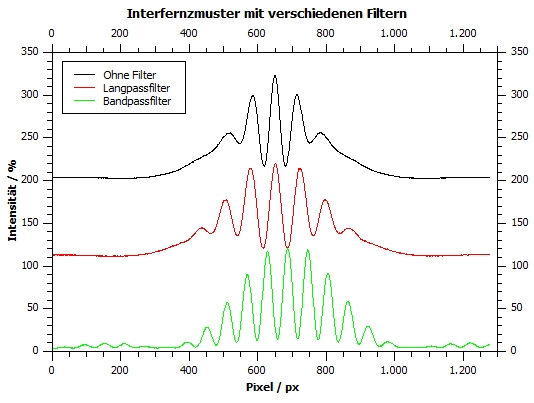
\includegraphics[width=0.6\linewidth]{nudes/aufgabe 2 plot.jpg}
    \caption{Interferenzmuster mit verschiedenen Filtern. Zur Darstellung wurden die Daten vertikal getrennt.}
    \label{fig:aufgabe 2 kontrast}
\end{figure}

\noindent
Wie man erkennen kann, sind mit den unterschiedlichen Filtern verschiedenen Intensitätsmaxima erkennbar. 
\\
Ohne Filter erkennt man 5 Intensitätsmaxima, mit Langpassfilter erkennt man 7 Intensitätsmaxima und mit dem Bandpassfilter erkennt man 11 Intensitätsmaxima. 
\\
\\
Man erkennt, dass bei einer kleineren spektralen Breite (durch die Filter) ein klareres Interferenzmuster sichtbar ist. 

\subsection{Teil 3}
Die aufgenommenen Interferenzmuster mit Substrat und Polyacrylat Schicht werden mit ImageJ analysiert und als CSV-Datei exportiert. 

\begin{figure}[H]
    \centering
    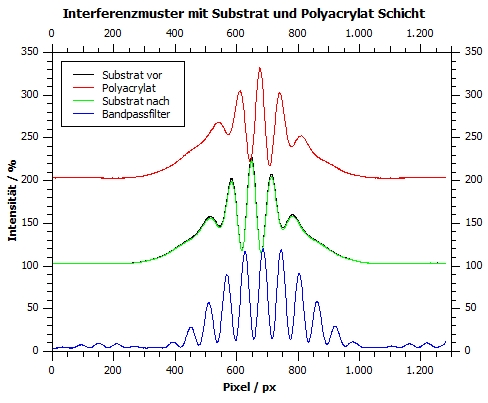
\includegraphics[width=0.6\linewidth]{nudes/aufgabe 3 plot.jpg}
    \caption{Interferenzmuster mit Substrat und Polyacrylat Schicht. Zur Darstellung wurden die Daten vertikal getrennt.}
    \label{fig:aufgabe 3 Interferenzmuster}
\end{figure}

\subsection{Teil 4}
Die Werte aus Tabelle \ref{tab:öffnungen} werden in einem Diagramm mit der theoretisch berechneten Kurve dargestellt. 

\begin{figure}[H]
    \centering
    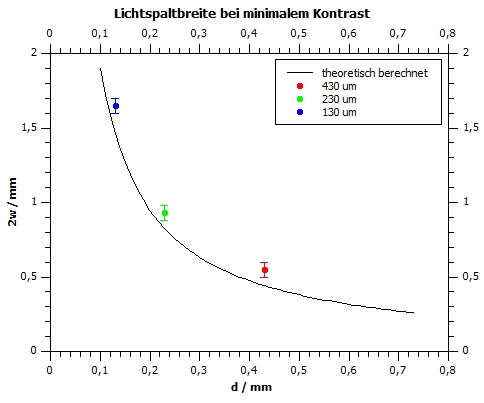
\includegraphics[width=0.6\linewidth]{nudes/aufgabe 4 plot.jpg}
    \caption{Lichtspaltbreite $2w$ bei minimalem Kontrast. Der theoretische Verlauf wird mit Formel \ref{eq:Kontrasttheorie} berechnet. }
    \label{fig:aufgabe 4 kontrast}
\end{figure}

\noindent
Wie man sehen kann, hat die kurve einen hyperbolischen Verlauf. Die Fehler fallen dabei bei den größeren Doppelspalten höher aus. 


\section{Diskussion} %diskussion der Unsicherheiten und Ergebnisse und evtl. verlgeich mit Literatur ------------------------------


\section{Zusammenfassung} %klare, übersichtliche vollständige beantwortung der Aufgabenstellung ------------------------------

 
\printbibliography[heading=bibintoc]
\end{document}
